The general equation of circle is represented as
\begin{align}
    \label{eq:solutions/4/1/3/circleeq}
    \vec{x}^T\vec{x}-2\vec{c}^T\vec{x}+f=0
\end{align}
where $\vec{c}$ is the center of the circle. Substituting the given points in the equation \eqref{eq:solutions/4/1/3/circleeq}, we obtain
\begin{align}
    \label{eq:solutions/4/1/3/points}
    2\myvec{2&3}\vec{c}-f=13\\
    2\myvec{3&2}\vec{c}-f=13\\
    2\myvec{5&1}\vec{c}-f=36
\end{align}
can be expressed in matrix form as 
\begin{align}
    \label{eq:solutions/4/1/3/matrix}
    \myvec{4&6&-1\\6&4&-1\\10&2&-1}\myvec{\vec{c}\\f}=\myvec{13\\13\\26}
\end{align}
\begin{figure}[!ht]
\centering
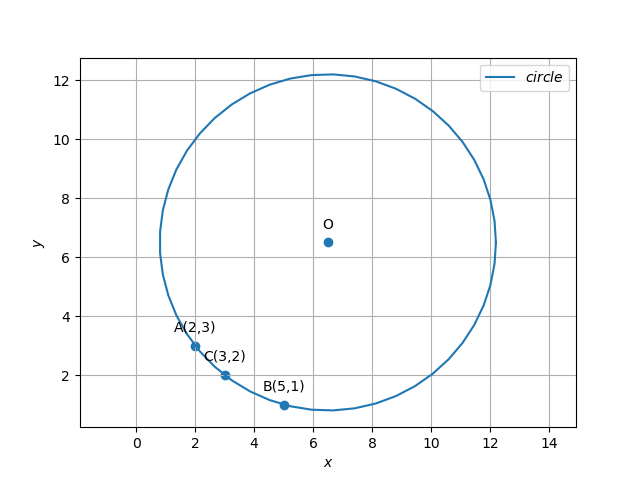
\includegraphics[width=\columnwidth]{./solutions/4/1/3/Circle.png}
\caption{Circle passing through the points A,B,C with center O}
\label{eq:solutions/4/1/3/fig1}
\end{figure}
The augmented matrix for \eqref{eq:solutions/4/1/3/matrix} can be row reduced as follows
\begin{align}
    \myvec{4&6&-1&13\\6&4&-1&13\\10&2&-1&26}\\
    \xleftrightarrow[R_2\leftarrow4R_2-6R_1]{R_3\leftarrow 4R_3-10R_1}
    \myvec{4&6&-1&13\\0&-20&2&-26\\0&-52&6&-26}\\
    \xleftrightarrow[]{R_3\leftarrow 5R_3-13R_2}
    \myvec{4&6&-1&13\\0&-20&2&-26\\0&0&4&208}\\
    \xleftrightarrow[R_1\leftarrow 4R_1+R_3]{R_2\leftarrow 2R_2-R_3}
   \myvec{16&24&0&260\\0&-40&0&-260\\0&0&4&208}\\
   \xleftrightarrow[]{R_1\leftarrow 5R_1+3R_2}
   \myvec{80&0&0&520\\0&-40&0&-260\\0&0&4&208}\\
   \label{eq:solutions/4/1/3/red}
   \xleftrightarrow[R_1\leftarrow \frac{R_1}{40}]{R_2\leftarrow\frac{R_2}{-20},R_3\leftarrow\frac{R_3}{4}}
   \myvec{2&0&0&13\\0&2&0&13\\0&0&1&52}
\end{align}
From the matrix \eqref{eq:solutions/4/1/3/red},
\begin{align}
    \vec{c}=\myvec{\frac{13}{2}\\\frac{13}{2}}\\
    k=52\\
    r=\sqrt{\norm{\vec{c}}^2-f}=11
\end{align}
Hence the circle equation can be written as,
\begin{align}
    \vec{x}^T\vec{x}-2\myvec{\frac{13}{2}&\frac{13}{2}}^T\vec{x}+52=0
\end{align}
